\documentclass{article}
\usepackage[paperwidth=20cm, paperheight=2cm, margin = 0cm, top=0.5cm]{geometry}

\usepackage{pgf}
\usepackage{tikz}
\usetikzlibrary{arrows,automata}

\tikzstyle{source}  = [draw,circle,fill=black,thick,inner sep=0mm,minimum size=2mm]

\begin{document}
\begin{center}
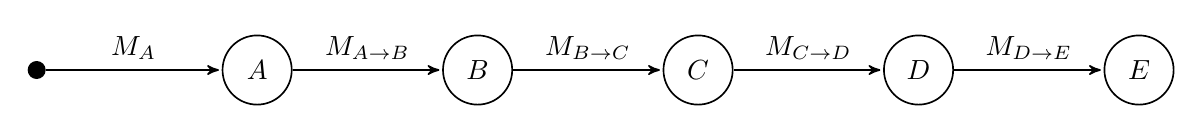
\begin{tikzpicture}[->,>=stealth',shorten >=1pt,auto,node distance=2.8cm,semithick]
                    
\node[source](X0)               {}; 
\node[state] (X1) [right of=X0] {$A$}; 
\node[state] (X2) [right of=X1] {$B$};                   
\node[state] (X3) [right of=X2] {$C$};                   
\node[state] (X4) [right of=X3] {$D$};                   
\node[state] (X5) [right of=X4] {$E$};                   

\path
    (X0) edge node {$M_{A}$}      (X1)  
	(X1) edge node {$M_{A\to B}$} (X2)
	(X2) edge node {$M_{B\to C}$} (X3)
	(X3) edge node {$M_{C\to D}$} (X4)
	(X4) edge node {$M_{D\to E}$} (X5);

\end{tikzpicture}
\end{center}

\end{document}
